\documentclass[tikz,border=6pt]{standalone}
\usepackage{pgfplots}
\pgfplotsset{compat=1.18}
\usepgfplotslibrary{colormaps}
\usetikzlibrary{arrows, arrows.meta, calc}
\usetikzlibrary{decorations.markings}


\usepackage{amssymb,amsmath,mathtools}

\usepackage[T1]{fontenc}
\usepackage[utf8]{inputenc}
\usepackage{newpxtext,newpxmath}
\usepackage{sectsty}

\renewcommand{\Re}{\operatorname{\mathrm{Re}}}
\renewcommand{\Im}{\operatorname{\mathrm{Im}}}

\begin{document}
	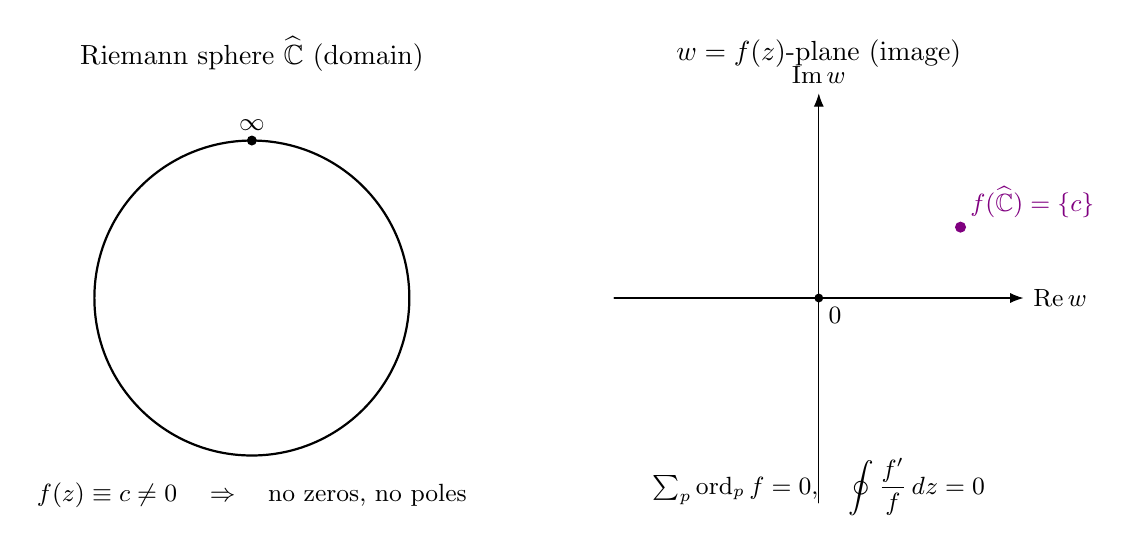
\begin{tikzpicture}[>=Latex, line cap=round, line join=round, font=\small]
		
		% ===== Left: Riemann sphere (stereographic view) =====
		\begin{scope}
			\node[font=\normalsize] at (0,3.1) {Riemann sphere $\widehat{\mathbb C}$ (domain)};
			% sphere silhouette
			\draw[thick] (0,0) circle (2.0);
			% mark infinity
			\fill (0,2.0) circle(1.8pt) node[above] {$\infty$};
			\node at (0,-2.5) {$f(z)\equiv c\neq 0 \quad\Rightarrow\quad \text{no zeros, no poles}$};
		\end{scope}
		
		% ===== Right: w-plane image =====
		\begin{scope}[shift={(7.2,0)}]
			\node[font=\normalsize] at (0,3.1) {$w=f(z)$-plane (image)};
			\draw[->] (-2.6,0)--(2.6,0) node[right] {$\Re w$};
			\draw[->] (0,-2.6)--(0,2.6) node[above] {$\Im w$};
			\fill (0,0) circle (1.6pt) node[below right] {$0$};
			% image is a single point c
			\coordinate (C) at (1.8,0.9);
			\fill[violet] (C) circle(2.0pt);
			\node[violet,above right] at (C) {$f(\widehat{\mathbb C})=\{c\}$};
			\node at (0,-2.4) {$\sum_p \operatorname{ord}_p f = 0,\quad \displaystyle\oint \frac{f'}{f}\,dz = 0$};
		\end{scope}
		
	\end{tikzpicture}
\end{document}
